
{
    Figure \ref{fig:rotation_test} is the outcome of the rotation test where some ants representatives from the test ground truth are rotated and compared with the original detection and a random detection from another identity. 
    It consist in two polar plots with a characterization of the cosine distance applied on the appearance descriptors. 
}

{
    The left plot, when one crop of one ant is compared with itself, serves to demonstrate the non-invariability over rotation. 
    Without taking into account the 0º rotation with the expected distance 0, the distance is clearly higher at \textpm90º of rotation. 
    However, the fact that a 180º rotation contains another minimum suggests a future research direction: the usage of a body alignment algorithms in inference that allow solutions with a 180º rotation.
}

\begin{figure}[!hp]
    \centering
    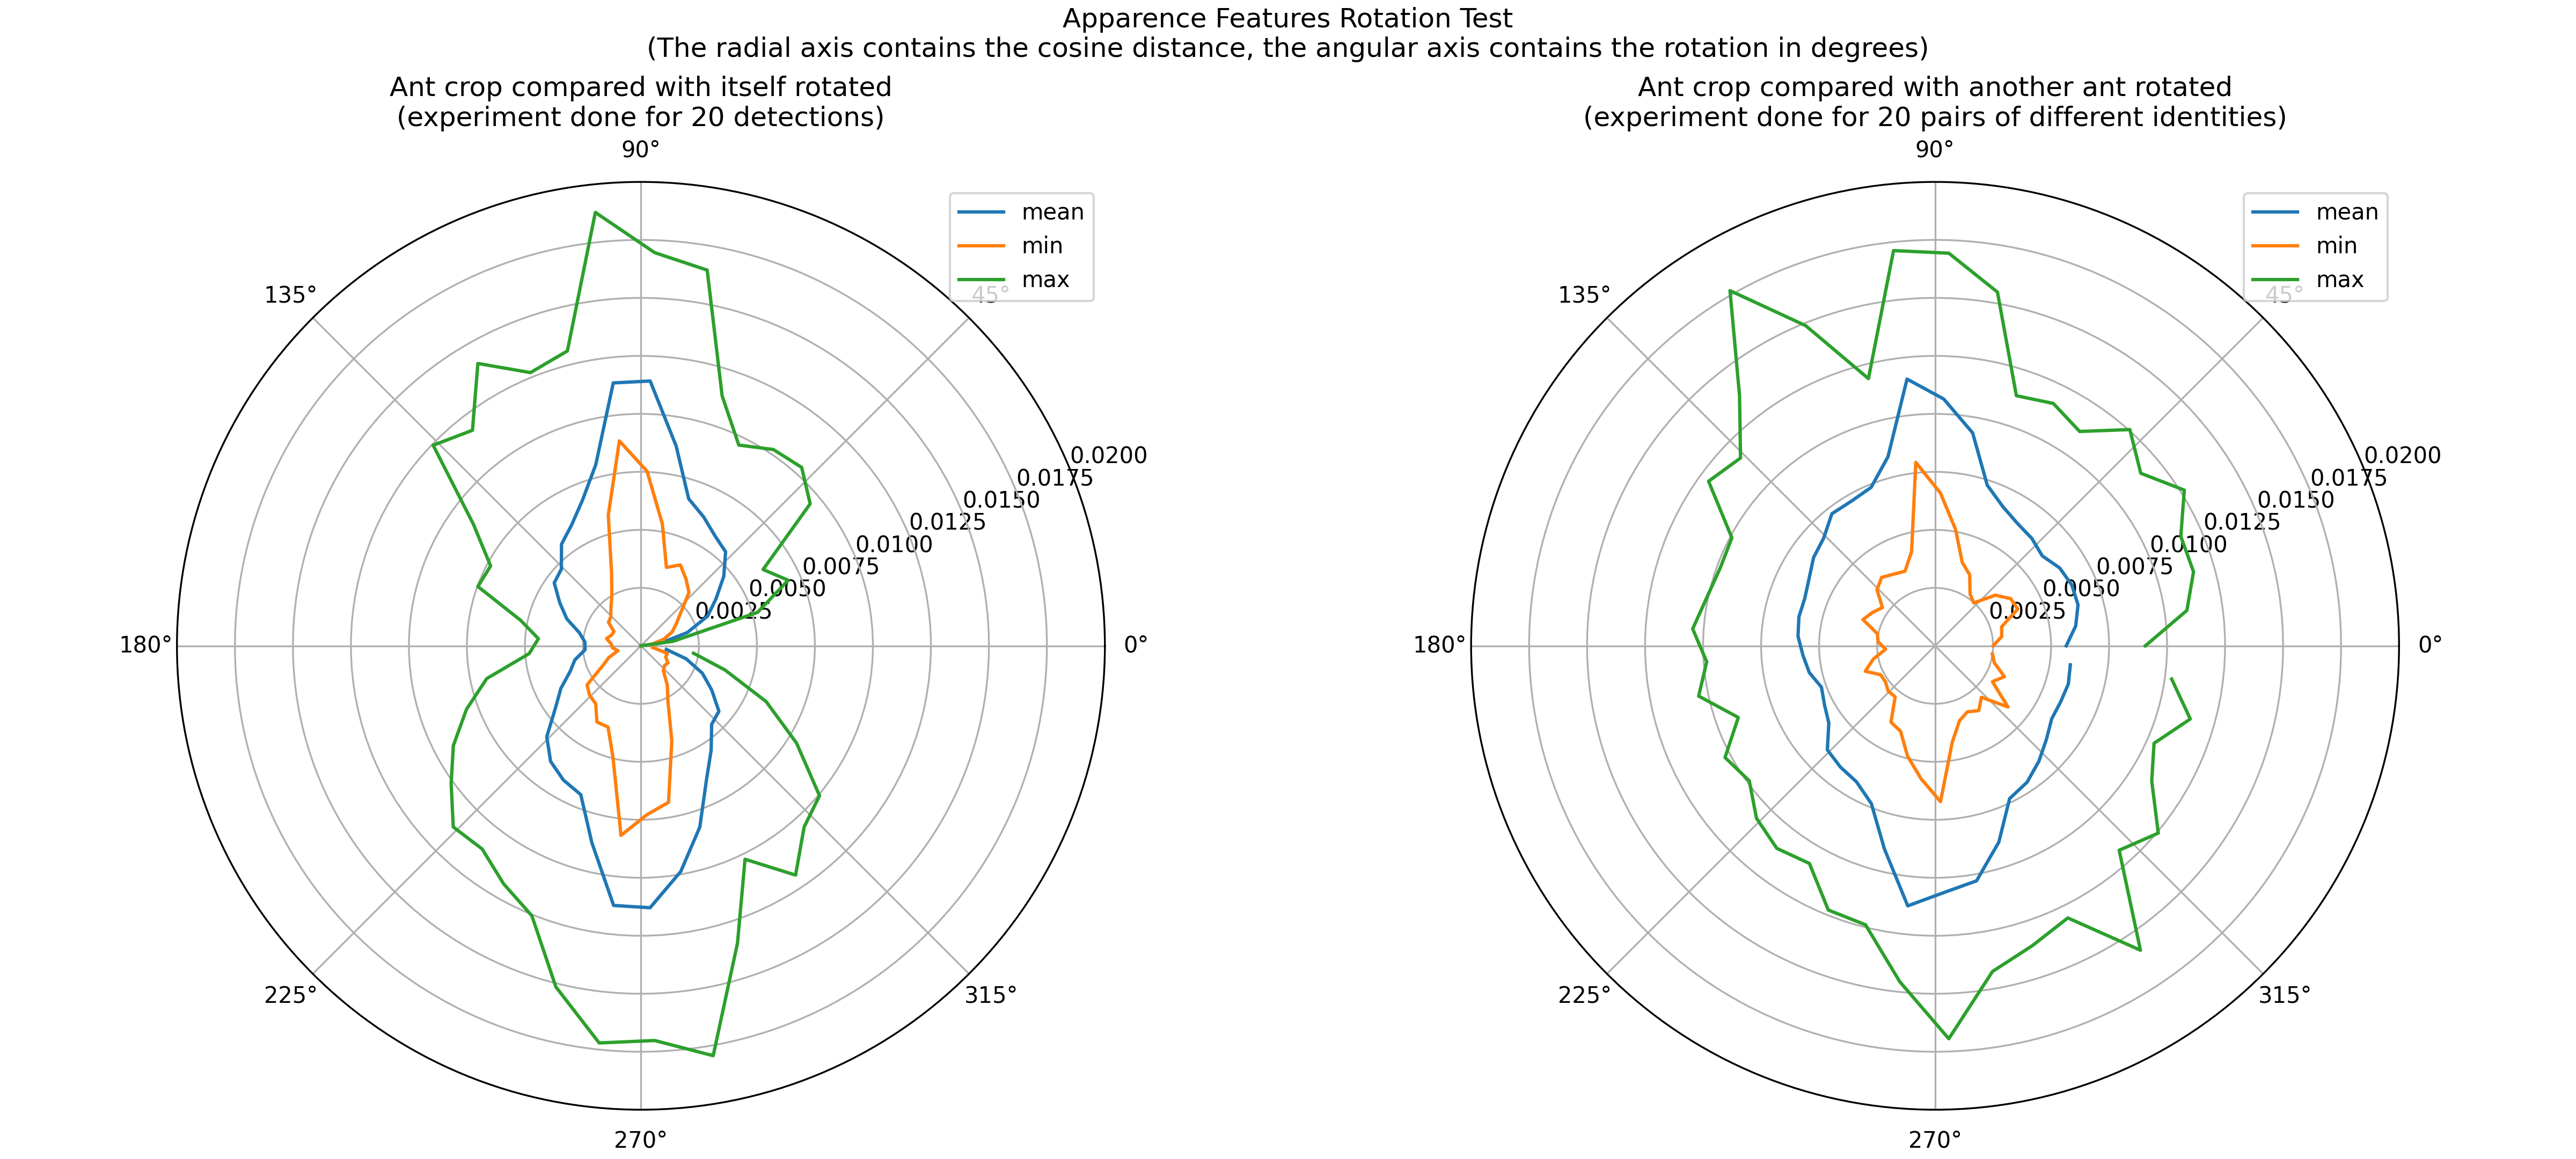
\includegraphics[width=0.8\textwidth]{figures/06_results/atr/rotation_all_ants_0-007.png}
    \caption[Appearance features rotation test]{\footnotesize{Validation of the rotation invariability property of the trained appearance features.}}
    \label{fig:rotation_test}
    \vspace{-1.5em}
\end{figure}

{
    The right plot of Figure \ref{fig:rotation_test}, when compared with the left plot, may provide an idea of the associability between tracks. 
    A 90º rotation makes one image as distant from itself as to another one. 
    However, to gain a clearer understanding, using the right plot to complement Figures \ref{fig:appearance_joinability} yields a clearer explanation.
}

{
    Figure \ref{fig:appearance_joinability_scope} depics the likelihood of correctly associating points where appearance is the most important feature: 
    the frames where ants are near each other. 
    When Figure \ref{fig:rotation_test} is examined, the tail of the probability density function for incorrect matches in Figure \ref{fig:appearance_joinability_scope} mainly contains distances related to a near 90º rotation of an ant with itself. 
}

{
    Figure \ref{fig:occlusion_scope} provides the ant displacement and duration of the instances where some ant is near another one.
    Most of these instances are short meetings within a small spatial scope, 
    this means that the most usual case is a small angular displacement because the ant did not have the time to rotate, 
    the better cases depicted in Figure \ref{fig:rotation_test}.
}

{
    Figure \ref{fig:appearance_joinability_all} exposes the distribution of means of distances for split tracklets within a single track and their comparison with tracklets from other tracks. 
    It is remarkable that the distributions are normalized in total area; in a real scenario, the problem tends to be unbalanced, with more negative cases than positives.   
}

\enlargethispage{1\baselineskip}

{
    It can be concluded that the appearance features are not usable yet, however, further research in this topic will still be relevant.
}

\begin{figure}[!hp]
	\centering
	\begin{subfigure}[]{0.49\textwidth}
		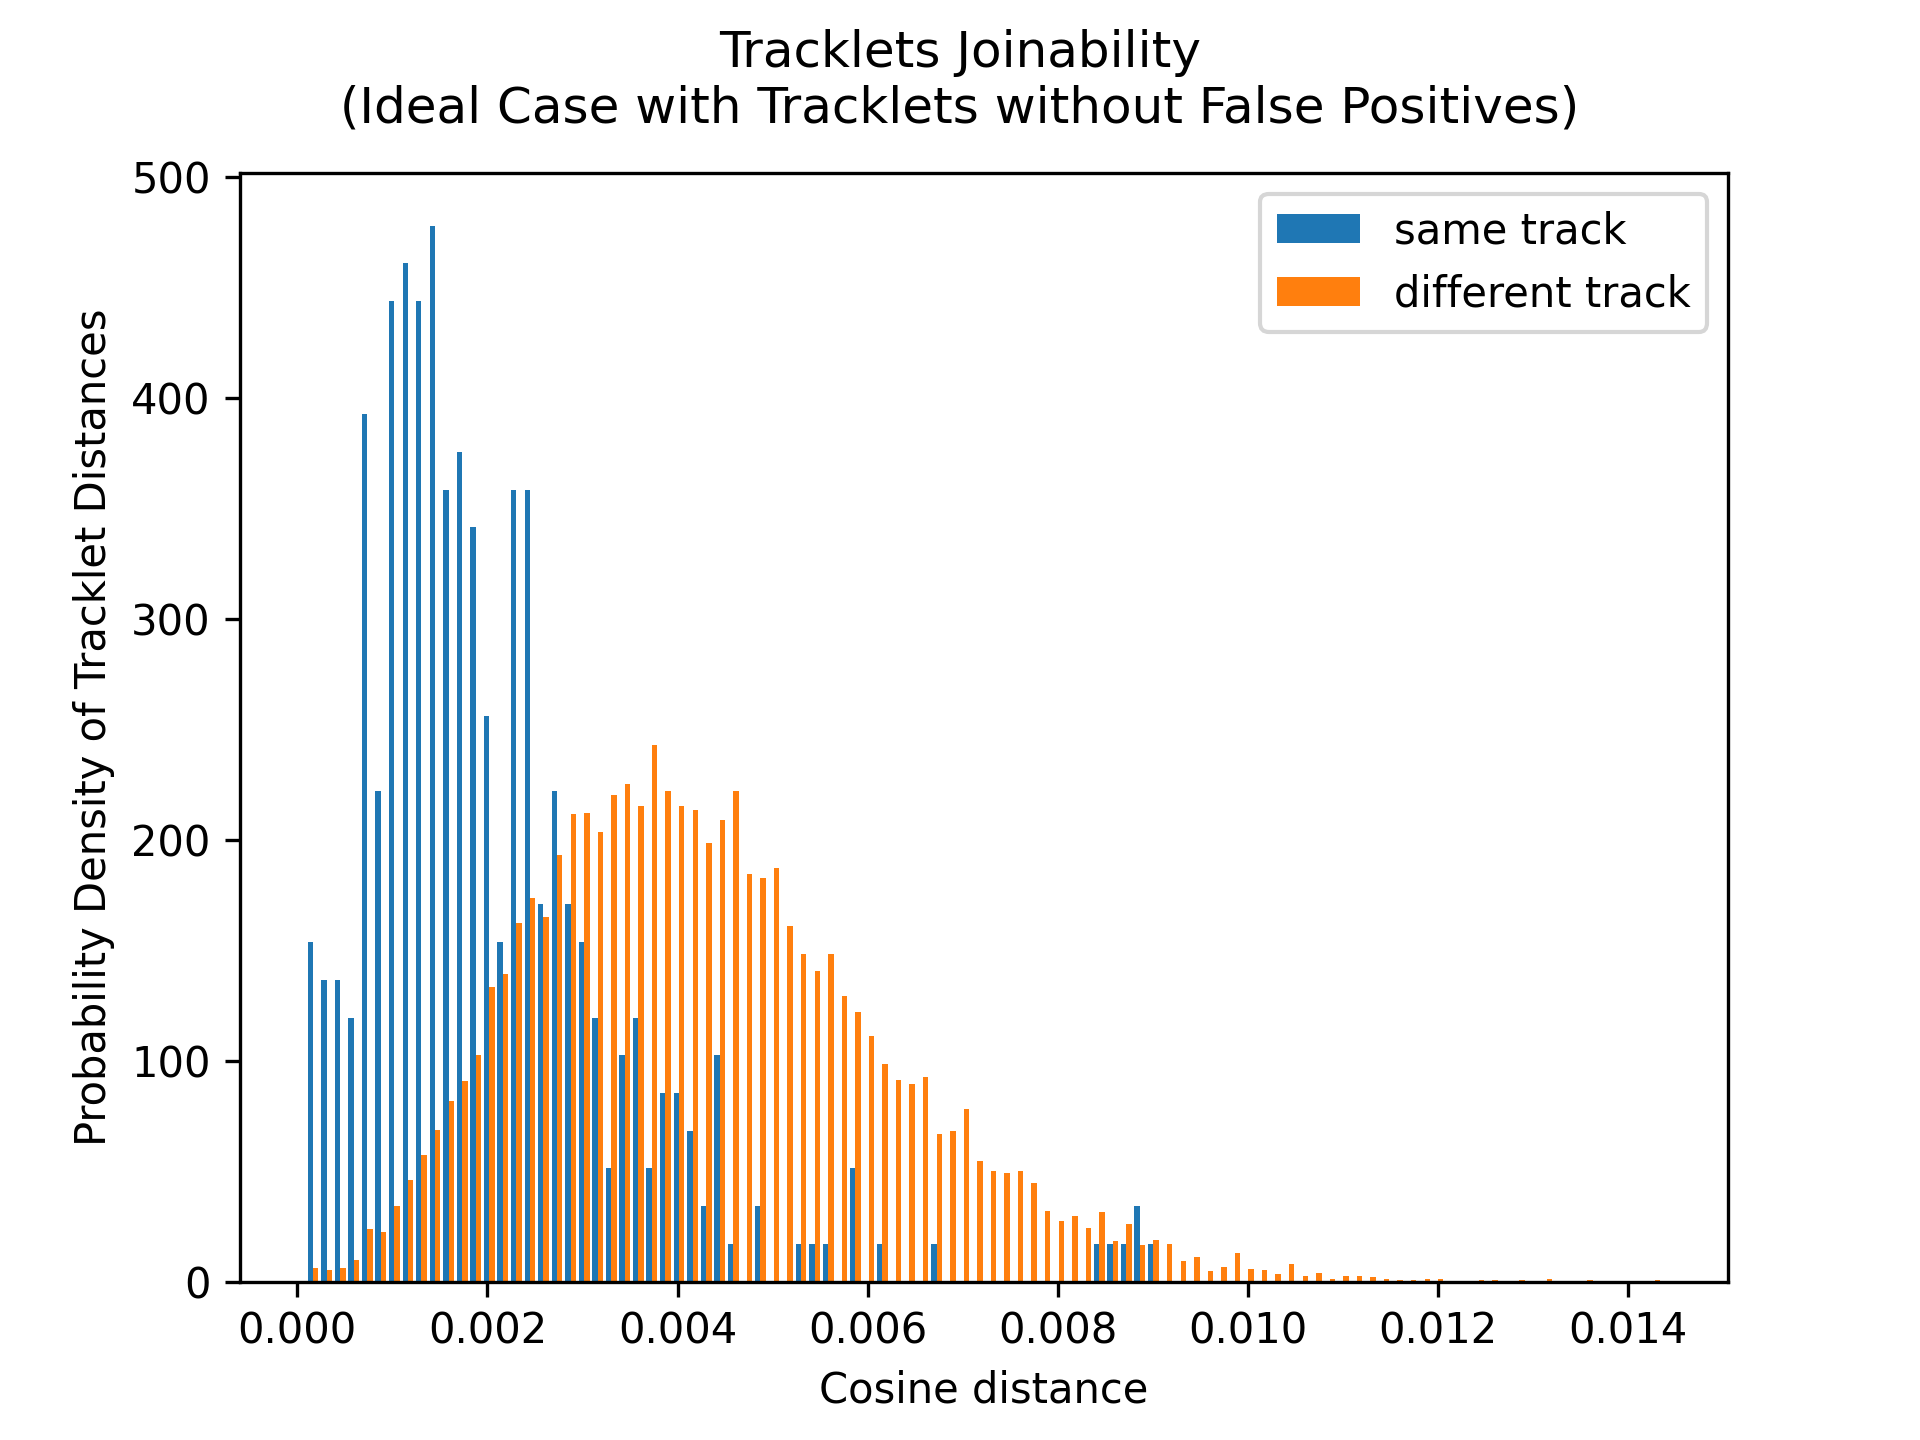
\includegraphics[width=\textwidth]{figures/06_results/atr/03_tracklet_dist_hist.png}
		\caption{\footnotesize{Normalized density function to determine the viability of an appearance model that fuse tracklets by their mean descriptor.}}
		\label{fig:appearance_joinability_all}
	\end{subfigure}
	\begin{subfigure}[]{0.49\textwidth}
		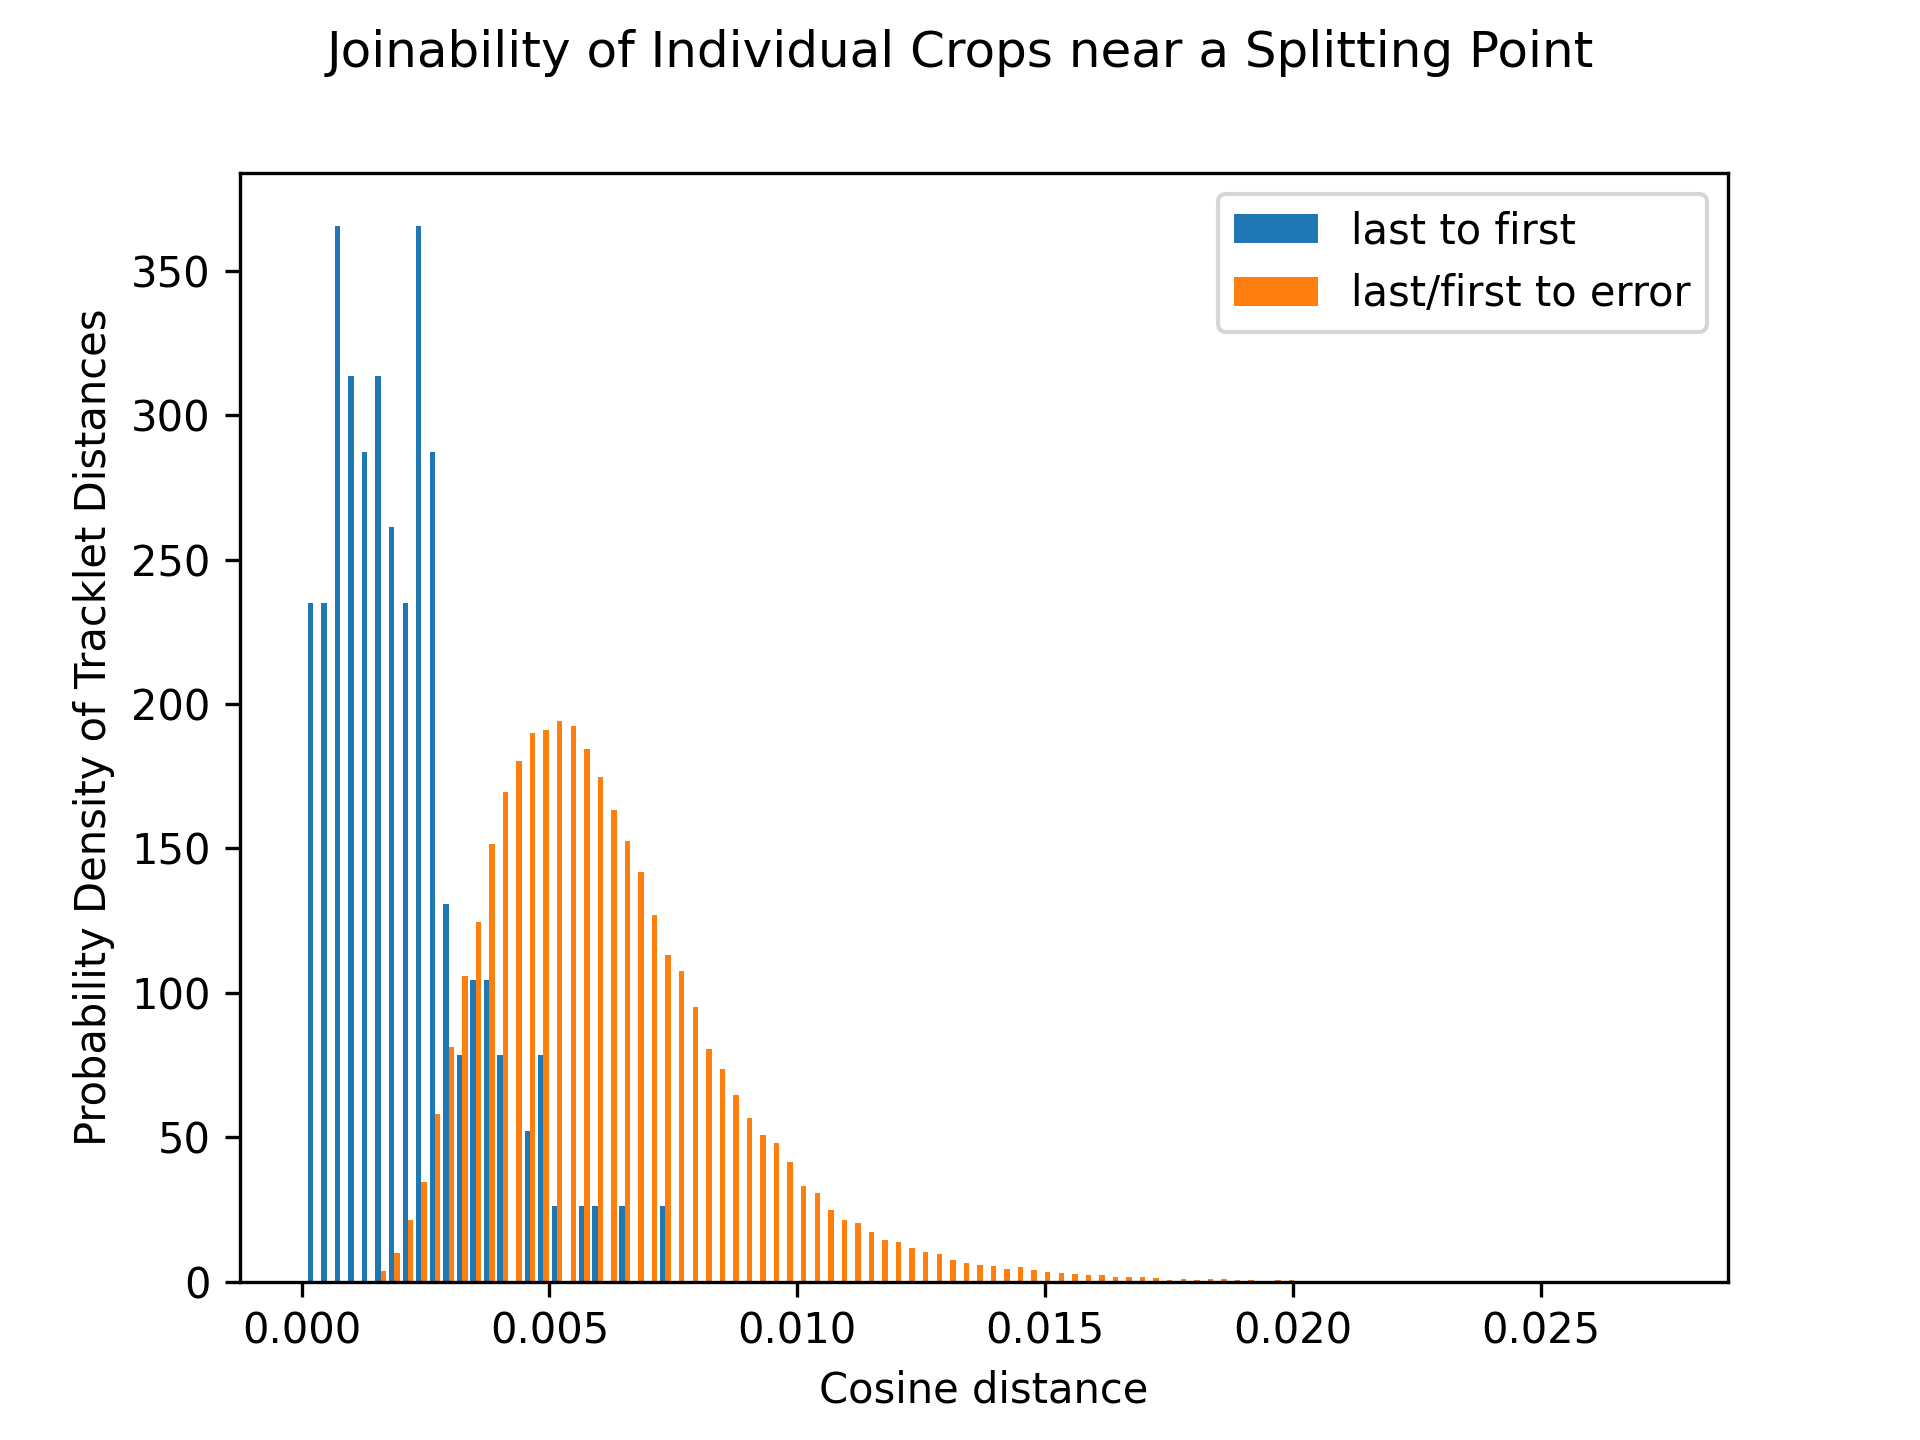
\includegraphics[width=\textwidth]{figures/06_results/atr/05_split_dist_hist.png}
		\caption{\footnotesize{Normalized density function to determine the viability of an appearance model that fuse tracklets based on the last known detection.}}
		\label{fig:appearance_joinability_scope}
	\end{subfigure}
	\caption[Appearance features associability]{\footnotesize{Appearance features associability tests obtained by analysising the ground truth with a split version of itself.}}
	\label{fig:appearance_joinability}
\end{figure}

\begin{figure}[!hp]
    \centering
    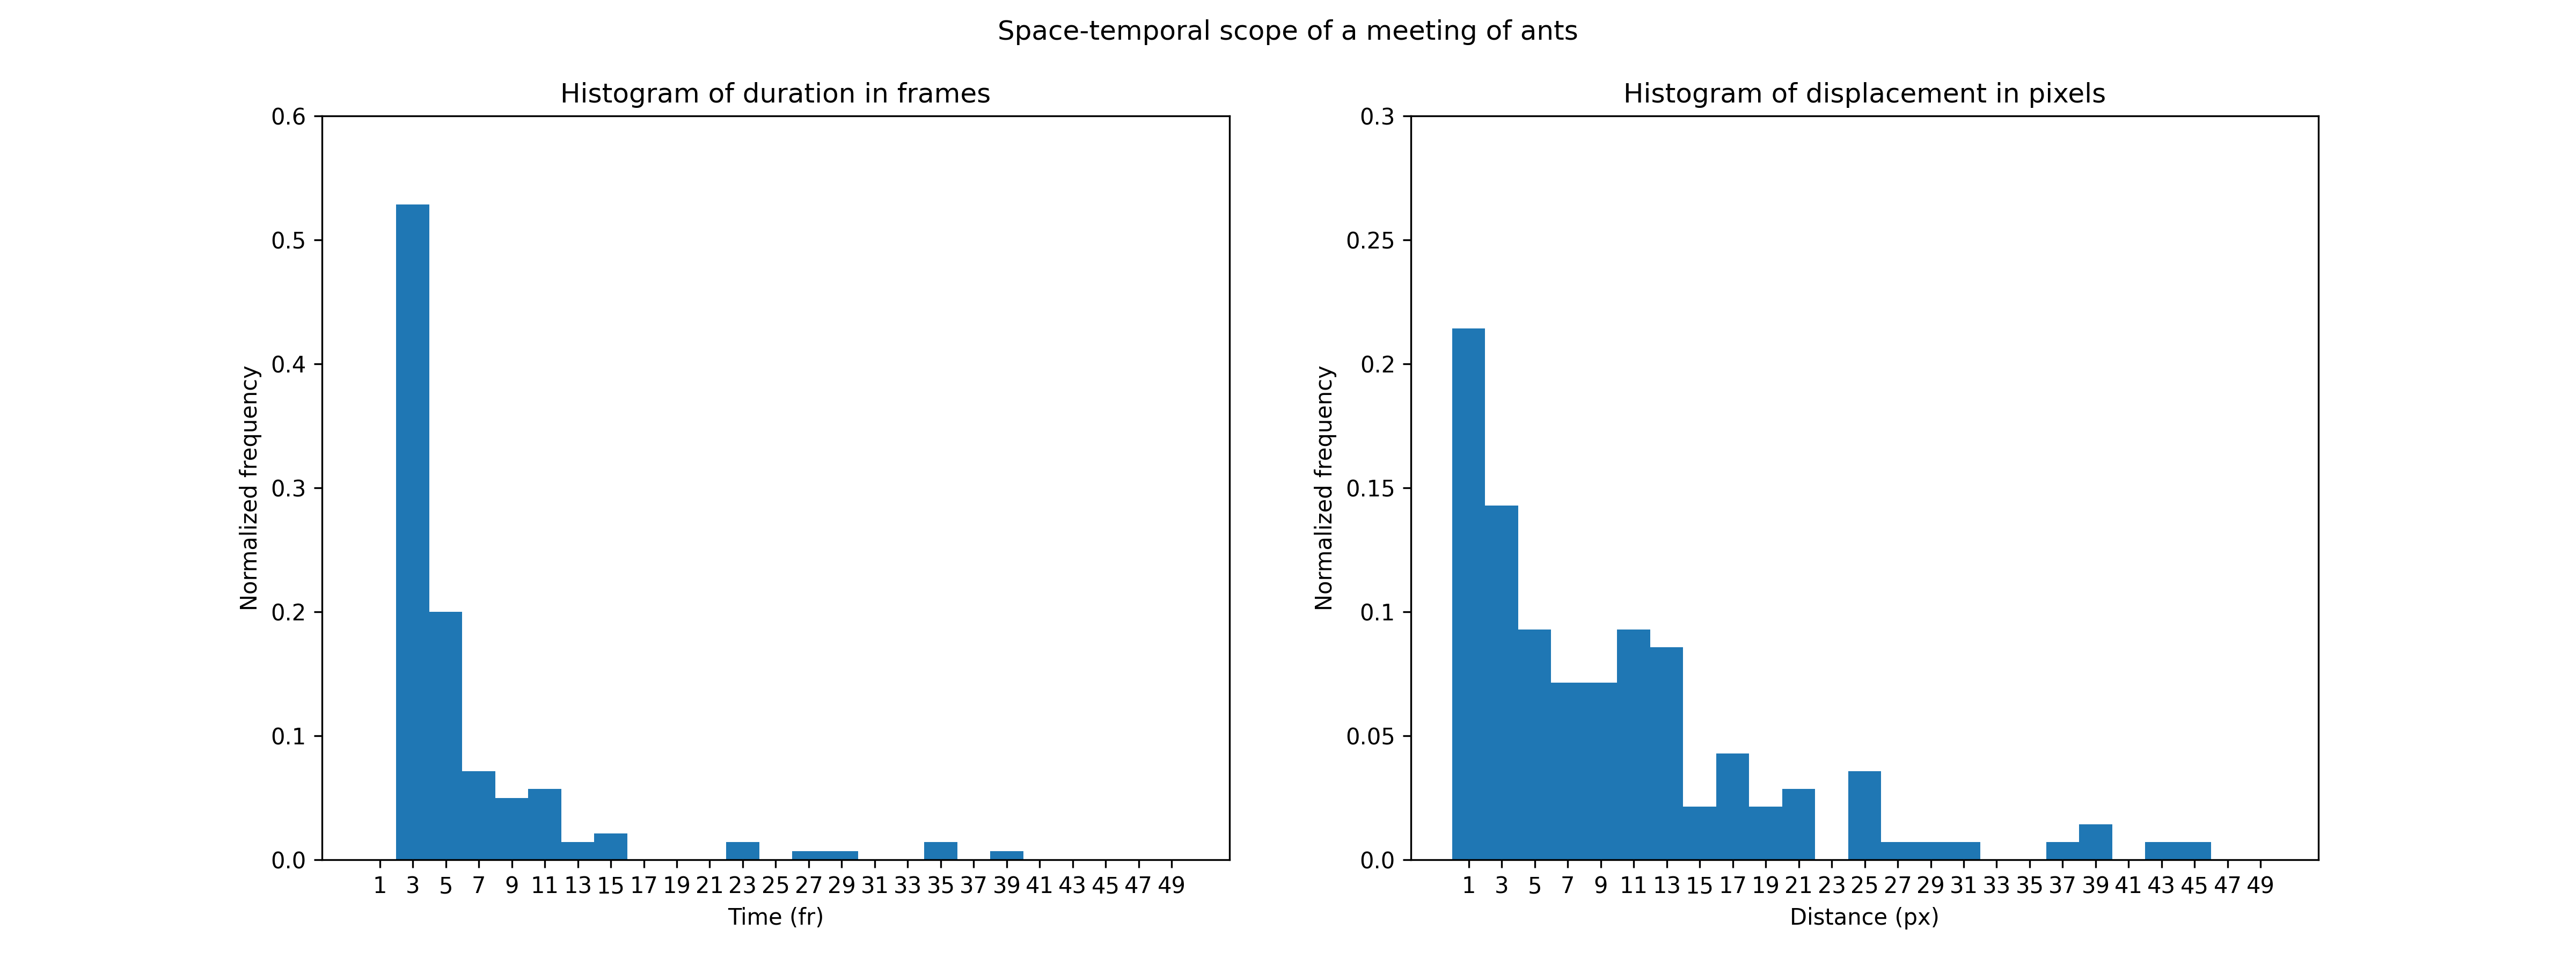
\includegraphics[width=\textwidth]{figures/06_results/atr/04_split_scope_hist.png}
    \caption[Analysis of the occlusions]{\footnotesize{Analysis of the temporal and spatial scope of the occlusions.}}
    \label{fig:occlusion_scope}
\end{figure}
